% ====================================================================
%  SECCIÓN 7 — ANÁLISIS DE REQUERIMIENTOS FUNCIONAL
% ====================================================================
\section{Análisis de Requerimientos Funcional}

\subsection{Actores}
\textbf{SuperAdmin:} usuario responsable de la administración de la plataforma. Gestiona la creación, habilitación y deshabilitación de cuentas de Administrador, transfiere el rol SuperAdmin cuando corresponde, administra el catálogo de empresas y ejecuta la ingesta de documentos.

\medskip
\textbf{Administrador:} usuario operativo responsable de consultar el asistente RAG, revisar las citas y resultados del análisis GRI, asignar manualmente los estados de los códigos detectados y generar reportes de prospección.

\medskip
\textbf{Proveedor de IA (Externo):} servicio externo consumido \emph{vía API} que sustenta el motor RAG: generación de \emph{embeddings} (indexación semántica) y generación de respuestas a las consultas del Administrador.

\medskip
\textbf{Servicio de correo (Externo):} servicio de envío de correo electrónico utilizado para la recuperación de contraseña.

\subsection{Diagrama Caso de Uso y su Especificación}

\subsubsection{Listado de casos de uso}
\begin{itemize}[leftmargin=1.4em,itemsep=2pt,topsep=2pt]
  \item Casos de uso de la Empresa
\end{itemize}

\begin{center}
\begin{tabular}{|C{2.4cm}|L{9.2cm}|C{2.9cm}|}
\hline
\thd{CÓDIGO} & \thd{NOMBRE} & \thd{CU PADRE} \\
\hline
CU001 & Autenticación y Gestión de Sesión & --- \\
\hline
CU002 & Gestión de Usuarios & --- \\
\hline
CU003 & Ingesta de Documentos (memorias y reportes GRI) & --- \\
\hline
CU004 & Consulta al Asistente de IA (RAG) & --- \\
\hline
CU005 & Detección de Brechas GRI y Sanciones & CU003 \\
\hline
CU006 & Generación de Reportes de Prospección (PDF) & CU005 \\
\hline
CU007 & Auditoría de Eventos del Sistema & --- \\
\hline
CU008 & Gestión del Catálogo de Empresas & --- \\
\hline
\end{tabular}
\end{center}

% ------------------------------- CU001 -------------------------------
\newcommand{\frow}[2]{#1 & #2 \\ \hline}
\newcommand{\ficha}[1]{\begin{longtable}{|>{\columncolor{cellgray}\bfseries\RaggedRight\arraybackslash}p{3.3cm}|L{11.9cm}|}\hline #1 \end{longtable}}
\newcommand{\figframe}[2]{\begin{center}\fbox{\begin{minipage}{0.94\textwidth}\centering\vspace{4pt}{\small [ IMAGEN ] #1}\\[6pt]#2\vspace{4pt}\end{minipage}}\end{center}}
\newcommand{\figempty}[1]{\begin{center}\fbox{\begin{minipage}{0.94\textwidth}\centering\vspace{6pt}{\small [ IMAGEN ] #1}\vspace{6pt}\end{minipage}}\end{center}}

\clearpage
\subsubsection*{CU001: Autenticación y Gestión de Sesión}
\addcontentsline{toc}{subsubsection}{CU001: Autenticación y Gestión de Sesión}
\ficha{
\frow{Descripción}{Este caso de uso permite a los usuarios registrados (SuperAdmin y Administrador) iniciar una sesión segura en la plataforma mediante correo electrónico y contraseña. El sistema valida las credenciales contra los registros existentes, verifica que la cuenta esté habilitada, identifica el rol y establece una sesión autenticada mediante un token JWT firmado que incorpora la identidad de la cuenta y su rol vigente. El caso de uso abarca además la recuperación de contraseña mediante enlace seguro, el cambio de contraseña con sesión activa, el cierre de sesión y la expiración de la sesión por inactividad.}
\frow{Actores}{SuperAdmin\newline Administrador\newline Servicio de correo (externo)}
\frow{Precondiciones}{-- El sistema debe estar desplegado y operativo.\newline -- La cuenta debe estar registrada en la plataforma y habilitada.\newline -- La cuenta debe contar con un rol asignado (SuperAdmin o Administrador).\newline -- Para la recuperación de contraseña, el correo debe estar registrado y el servicio de correo disponible.}
\frow{Flujo Básico}{\textbf{Autenticación exitosa}\newline 1. El usuario accede a la URL de la plataforma. El sistema muestra el formulario de inicio de sesión.\newline 2. El usuario ingresa su correo electrónico y contraseña, y selecciona ``Iniciar sesión''.\newline 3. El sistema valida que la cuenta exista y se encuentre habilitada.\newline 4. El sistema valida que la contraseña corresponda a la cuenta registrada.\newline 5. El sistema identifica el rol de la cuenta (SuperAdmin o Administrador) y genera un token de autenticación firmado que incorpora la identidad y el rol vigente.\newline 6. El sistema establece la sesión activa y redirige al usuario a la vista principal correspondiente a su rol: panel de gestión para SuperAdmin, panel analítico para Administrador.}
\frow{Flujo Alternativo}{\textbf{Credenciales inválidas}\newline En el paso 4, la contraseña no corresponde a la cuenta. El sistema muestra el mensaje ``Credenciales inválidas'' ---idéntico tanto si la cuenta no existe como si la contraseña es incorrecta--- y el usuario permanece en la pantalla de inicio, donde puede reintentar.\par\vspace{4pt}\textbf{Correo con formato inválido}\newline En el paso 2, el usuario ingresa un correo con formato inválido. El sistema muestra ``Ingrese un correo válido.'' y no procesa la solicitud.\par\vspace{4pt}\textbf{Cuenta deshabilitada}\newline En el paso 3, el sistema detecta que la cuenta está deshabilitada. Bloquea el acceso y muestra ``Usuario deshabilitado''. Contacte al administrador.''\par\vspace{4pt}\textbf{Bloqueo por intentos fallidos}\newline Tras 5 intentos fallidos consecutivos, el sistema bloquea temporalmente la cuenta durante 15 minutos, impide nuevos intentos y registra el evento en el módulo de auditoría.\par\vspace{4pt}\textbf{Recuperación de contraseña}\newline 1. Desde la pantalla de inicio, el usuario selecciona ``¿Olvidaste tu contraseña?'' e ingresa el correo asociado a la cuenta.\newline 2. El sistema muestra un mensaje idéntico para toda cuenta (``Si el correo está registrado en el sistema, recibirás un enlace de recuperación en los próximos minutos''), genera un enlace seguro con vigencia de 30 minutos y lo envía por correo.\newline 3. El usuario abre el enlace, que lo redirige a la pantalla de recuperación, e ingresa y confirma una nueva contraseña que cumpla la política de seguridad.\newline 4. El sistema actualiza la contraseña, invalida el enlace utilizado y redirige al formulario de inicio de sesión.\newline Variantes: si el enlace expiró, el sistema muestra ``El enlace de recuperación ha expirado.'' y solicita generar uno nuevo; si las contraseñas no coinciden, muestra ``Las contraseñas no coinciden.''; si la contraseña no cumple los requisitos, muestra el mensaje con la política mínima. En ningún caso se actualiza la contraseña.\par\vspace{4pt}\textbf{Cambio de contraseña con sesión activa}\newline Un usuario autenticado cambia su propia contraseña. El sistema aplica la misma política de complejidad y almacenamiento seguro que en el registro.\par\vspace{4pt}\textbf{Cierre de sesión y expiración por inactividad}\newline El usuario puede cerrar sesión manualmente, con lo que el sistema invalida la sesión activa. Además, tras 2 horas de inactividad el sistema expira la sesión y solicita reautenticación. Si la cuenta es deshabilitada, todas sus sesiones activas se invalidan de inmediato; tras una transferencia del rol SuperAdmin, la sesión aplica el rol vigente.}
\frow{Post Condiciones}{-- Éxito: el usuario queda autenticado con una sesión activa y un token que refleja su rol vigente; solo se habilitan las funcionalidades correspondientes a su rol.\newline -- Fallo: el usuario permanece en la pantalla de inicio de sesión, sin acceso a la plataforma.}
\frow{Restricciones}{-- Solo pueden autenticarse las cuentas registradas y habilitadas en el sistema.\newline -- La identidad y la sesión se obtienen del token JWT firmado. El rol utilizado para autorizar la operación se consulta en la base de datos en cada petición, evitando utilizar un rol desactualizado almacenado en el token.\newline -- Las contraseñas se almacenan mediante una función de hash de un solo sentido con sal única por usuario; nunca se guardan en texto plano.\newline -- La autorización se evalúa en cada endpoint y la revocación de la sesión se verifica en cada petición.}
\frow{Casos de Uso Padre}{Ninguno}
}
\figframe{Diagrama de caso de uso --- CU001}{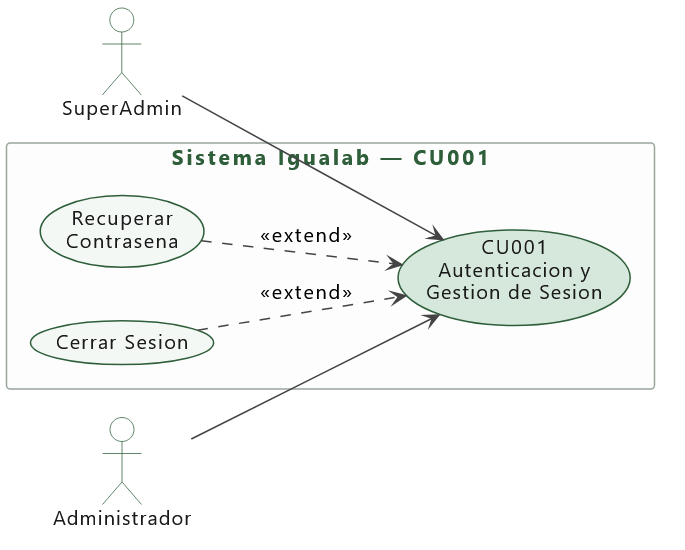
\includegraphics[width=0.78\textwidth]{img/im-019-011.png}}
\figframe{Prototipo --- CU001}{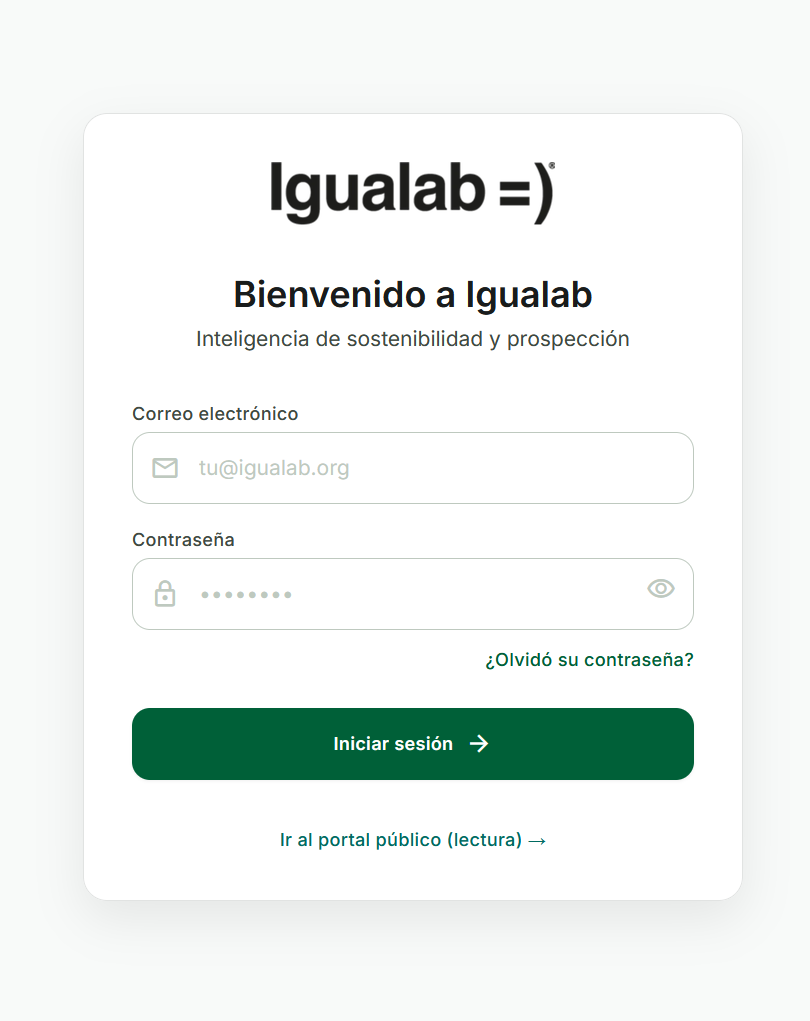
\includegraphics[width=0.52\textwidth]{img/im-020-012.png}}

% ------------------------------- CU002 -------------------------------
\clearpage
\subsubsection*{CU002: Gestión de Usuarios}
\addcontentsline{toc}{subsubsection}{CU002: Gestión de Usuarios}
\ficha{
\frow{Descripción}{Este caso de uso permite al SuperAdmin realizar la administración de las cuentas del sistema: crear cuentas (a las que se asigna automáticamente el rol Administrador), habilitar y deshabilitar cuentas de Administrador, listar las cuentas existentes con su rol y estado, y transferir el rol SuperAdmin a una cuenta de Administrador existente y habilitada. La transferencia es atómica y garantiza que en todo momento exista exactamente una cuenta SuperAdmin.}
\frow{Actores}{SuperAdmin}
\frow{Precondiciones}{-- El SuperAdmin debe haber iniciado sesión exitosamente.\newline -- Para crear una cuenta, el correo ingresado no debe estar registrado previamente.\newline -- Para transferir el rol SuperAdmin, la cuenta destino debe existir, tener rol Administrador y estar habilitada.}
\frow{Flujo Básico}{\textbf{Administración de cuentas}\newline 1. El SuperAdmin accede al módulo de gestión de usuarios.\newline 2. El sistema lista las cuentas existentes mostrando, para cada una, su nombre, correo, rol y estado (habilitada o deshabilitada).\newline 3. El SuperAdmin crea una cuenta ingresando nombre, correo y contraseña.\newline 4. El sistema valida que el correo no esté registrado, crea la cuenta y le asigna automáticamente el rol Administrador.\newline 5. El sistema confirma la creación y actualiza el listado de cuentas.}
\frow{Flujo Alternativo}{\textbf{Correo ya registrado}\newline En el paso 3, el correo ingresado ya existe en el sistema. El sistema rechaza el registro e informa que el correo ya está en uso.\par\vspace{4pt}\textbf{Habilitar / deshabilitar cuenta}\newline El SuperAdmin habilita o deshabilita una cuenta de Administrador. Al deshabilitarla, el sistema invalida de inmediato todas las sesiones activas de esa cuenta y le revoca el acceso a todas las funcionalidades.\par\vspace{4pt}\textbf{Intento de deshabilitar o eliminar al SuperAdmin}\newline El sistema impide deshabilitar o eliminar la cuenta con rol SuperAdmin desde la aplicación, indicando que primero debe transferirse el rol a otra cuenta.\par\vspace{4pt}\textbf{Transferencia del rol SuperAdmin}\newline 1. El SuperAdmin selecciona como destino una cuenta de Administrador existente y habilitada.\newline 2. El sistema muestra una alerta de confirmación antes de ejecutar el cambio.\newline 3. Al confirmar, el sistema ejecuta la transferencia de forma atómica: la cuenta destino adquiere el rol SuperAdmin y la cuenta origen pasa a rol Administrador en una sola operación. Las sesiones activas aplican el rol vigente tras la transferencia.\par\vspace{4pt}\textbf{Transferencia inválida}\newline Si la cuenta destino no existe, está deshabilitada o ya tiene rol SuperAdmin, el sistema rechaza la transferencia e informa el motivo.}
\frow{Post Condiciones}{-- Éxito: las cuentas y sus estados o roles quedan persistidos; el sistema mantiene siempre exactamente una cuenta con rol SuperAdmin.\newline -- Fallo: la operación se cancela y se notifica el error, sin alterar el estado de las cuentas.}
\frow{Restricciones}{-- Solo el rol SuperAdmin puede acceder a este módulo.\newline -- En todo momento existe exactamente una cuenta con rol SuperAdmin, con independencia de su estado o de que tenga una sesión abierta; esto se garantiza además mediante una restricción de integridad en la base de datos.\newline -- La cuenta SuperAdmin inicial se crea durante el despliegue y no puede crearse desde la aplicación.\newline -- Toda cuenta creada desde la aplicación nace con rol Administrador; el rol SuperAdmin solo se obtiene por transferencia.\newline -- La transferencia del rol se ejecuta dentro de una transacción única; un fallo parcial revierte toda la operación.}
\frow{Casos de Uso Padre}{---}
}
\figframe{Diagrama de caso de uso --- CU002}{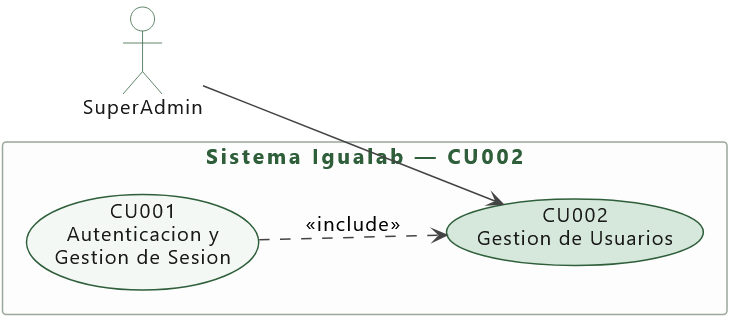
\includegraphics[width=0.72\textwidth]{img/im-022-013.png}}
\figframe{Prototipo --- CU002}{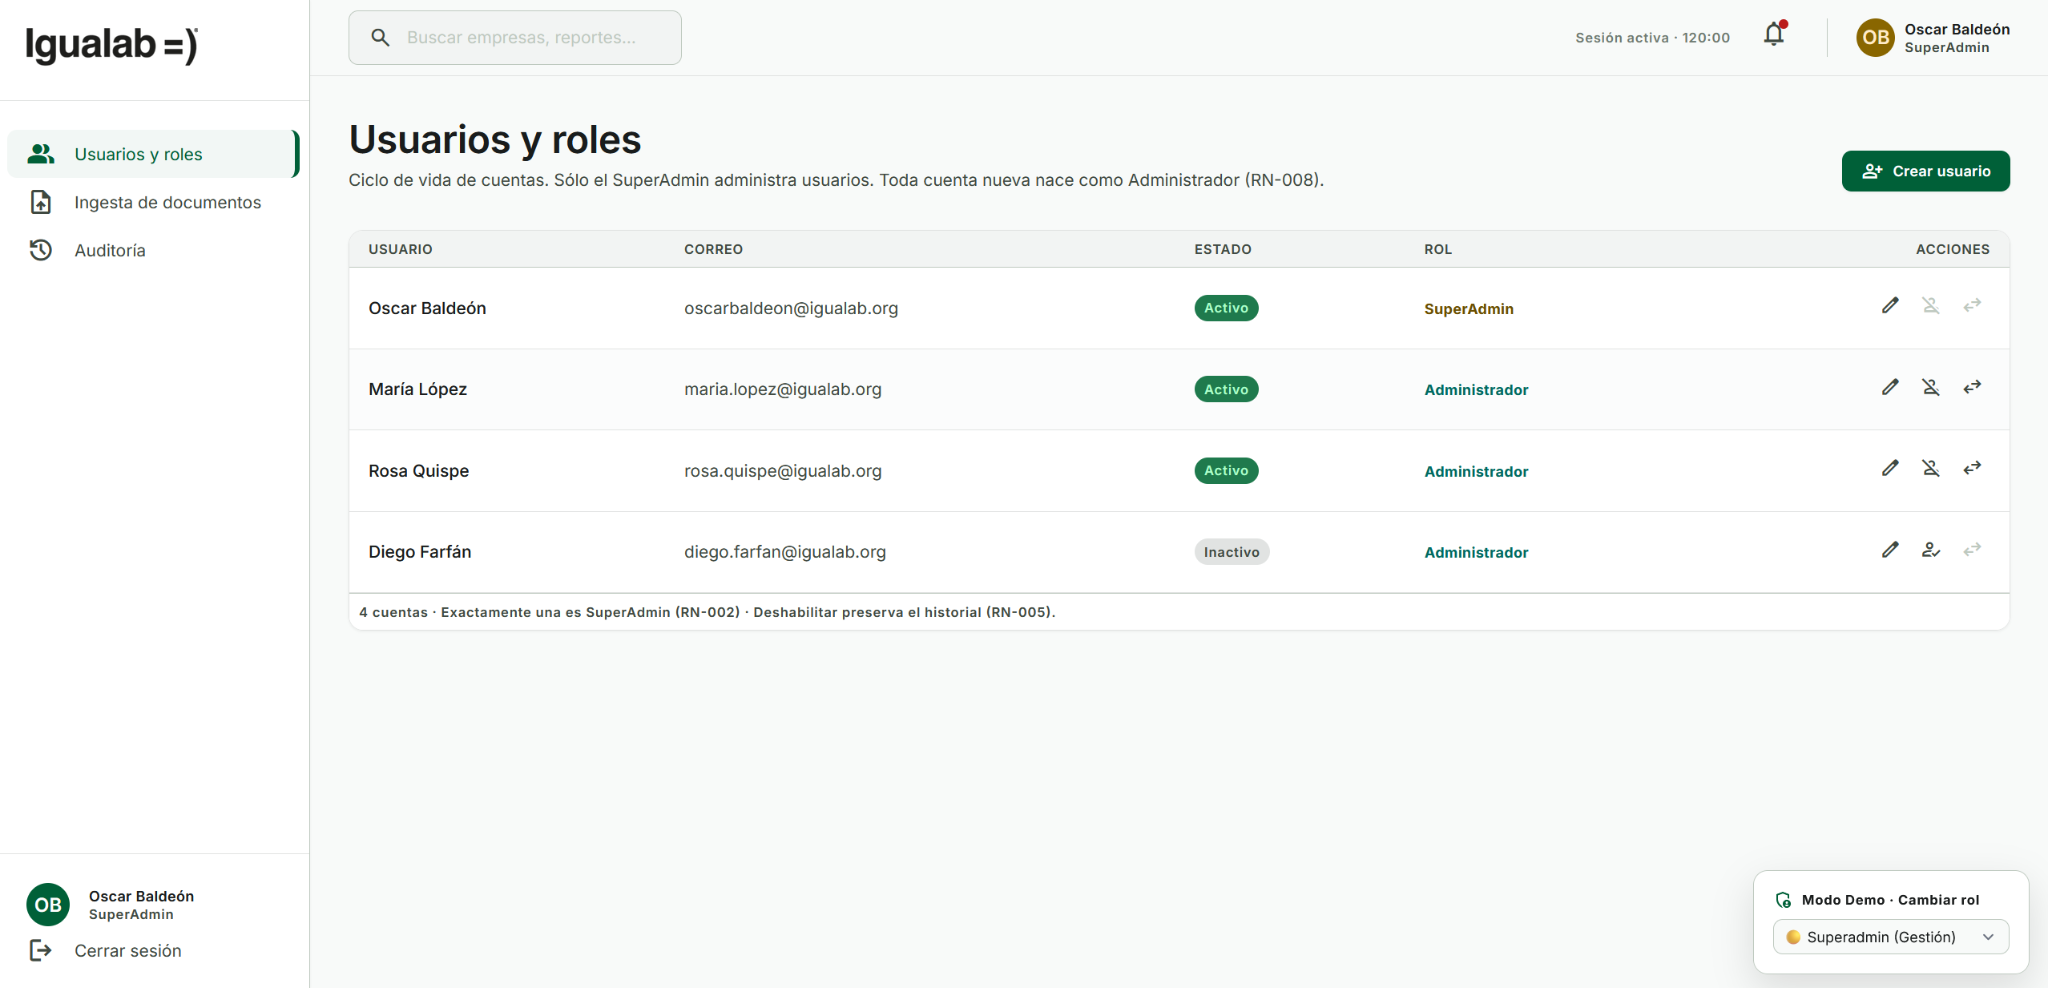
\includegraphics[width=0.9\textwidth]{img/im-022-014.png}}
\figframe{Prototipo --- CU002}{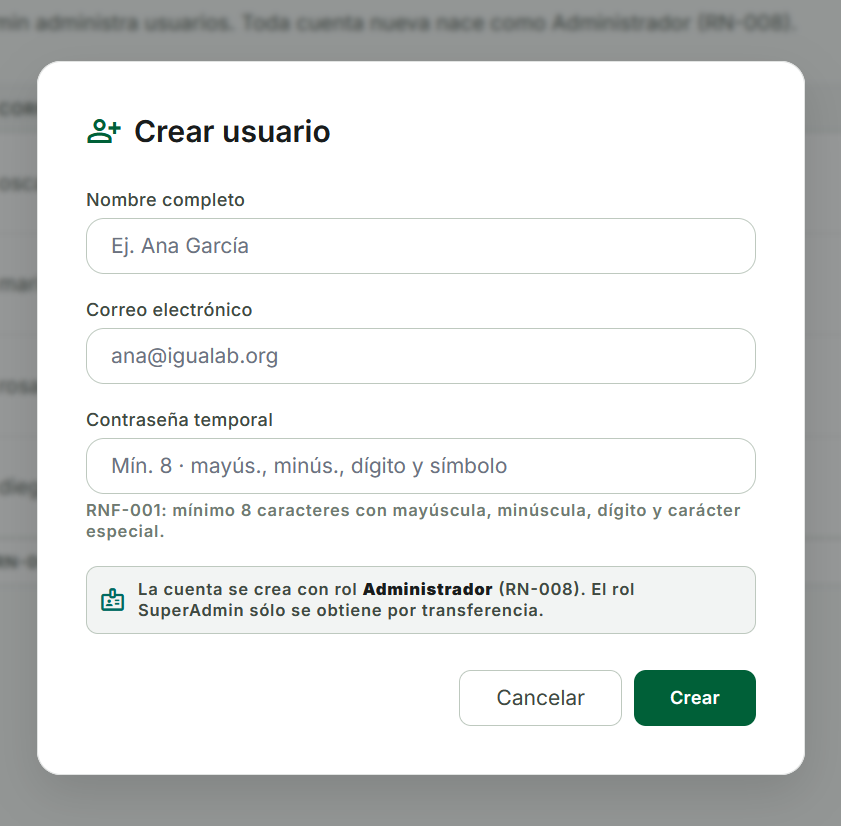
\includegraphics[width=0.62\textwidth]{img/im-023-016.png}}

% ------------------------------- CU003 -------------------------------
\clearpage
\subsubsection*{CU003: Ingesta de Documentos (memorias y reportes GRI)}
\addcontentsline{toc}{subsubsection}{CU003: Ingesta de Documentos (memorias y reportes GRI)}
\ficha{
\frow{Descripción}{Este caso de uso permite al SuperAdmin cargar memorias anuales y reportes de sostenibilidad GRI en formato Markdown (.md, con tablas de pipes), asociándolos a una empresa, un año y un tipo. El sistema valida el archivo, calcula su hash para evitar duplicados, lo indexa para el asistente y ejecuta automáticamente el análisis GRI como último paso.}
\frow{Actores}{SuperAdmin}
\frow{Precondiciones}{-- El SuperAdmin debe haber iniciado sesión exitosamente.\newline -- Debe existir la empresa (activa) a la que se asociará el documento.\newline -- El archivo debe estar en Markdown (.md), con tablas de pipes y un tamaño de hasta 50 MB.}
\frow{Flujo Básico}{\textbf{Ingesta de documentos}\newline 1. El SuperAdmin accede al módulo de Ingesta de documentos.\newline 2. Selecciona el sector y la empresa, el año y el tipo (memoria anual o reporte de sostenibilidad GRI).\newline 3. Selecciona el archivo .md y pulsa ``Ingestar''.\newline 4. El sistema valida el tipo real del archivo, el tamaño (hasta 50 MB), las tablas con pipes y el contenido mínimo (al menos un código GRI o una mención de sanción).\newline 5. El sistema calcula el hash SHA-256 y verifica la unicidad (por contenido y por empresa/año/tipo).\newline 6. El sistema procesa el documento de forma síncrona: parseo, segmentación (chunking), embeddings por API e indexación.\newline 7. Al finalizar la indexación, ejecuta el análisis GRI y de sanciones (las filas quedan sin estado, pendientes de validación humana).\newline 8. El sistema muestra el resultado (número de fragmentos indexados o el estado) y registra el evento en la auditoría.}
\frow{Flujo Alternativo}{\textbf{Empresa no registrada}\newline Si la empresa no existe, el SuperAdmin puede crearla con ``Agregar empresa'' ingresando su nombre y su sector, y reintentar la ingesta.\par\vspace{4pt}\textbf{Documento duplicado}\newline Si el contenido ya fue ingestado (mismo hash) o ya existe un documento del mismo tipo para la empresa y el año, el sistema rechaza la carga e indica la fecha y la cuenta de la carga original.\par\vspace{4pt}\textbf{Documento sin contenido analizable}\newline Si el documento no contiene ningún código GRI ni mención de sanción, el sistema lo marca como \emph{observado} (no rechazado) y no lo indexa hasta corregirse.\par\vspace{4pt}\textbf{Rechazo o interrupción}\newline Si el archivo no es .md, supera los 50 MB o el proceso se interrumpe, el sistema revierte el procesamiento (sin dejar fragmentos, embeddings ni análisis parciales) y conserva solo el motivo del rechazo.}
\frow{Post Condiciones}{-- Éxito: el documento queda indexado y el análisis GRI/sanciones poblado, listo para la revisión del Administrador.\newline -- Fallo: el documento queda como rechazado u observado con su motivo, sin incorporar contenido al corpus.}
\frow{Restricciones}{-- Solo el rol SuperAdmin puede acceder a este módulo.\newline -- Solo se admite Markdown (.md) con tablas de pipes; el sistema no convierte formatos.\newline -- Tamaño máximo por archivo: 50 MB.\newline -- La ingesta es atómica: no deja contenido parcial ante rechazo o interrupción.}
\frow{Casos de Uso Padre}{---}
}
\figframe{Diagrama de caso de uso --- CU003}{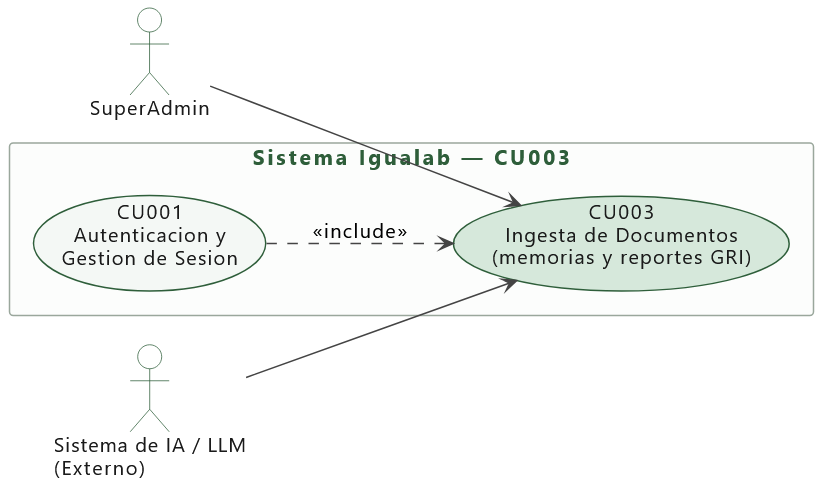
\includegraphics[width=0.72\textwidth]{img/im-025-018.png}}
\figframe{Prototipo --- CU003}{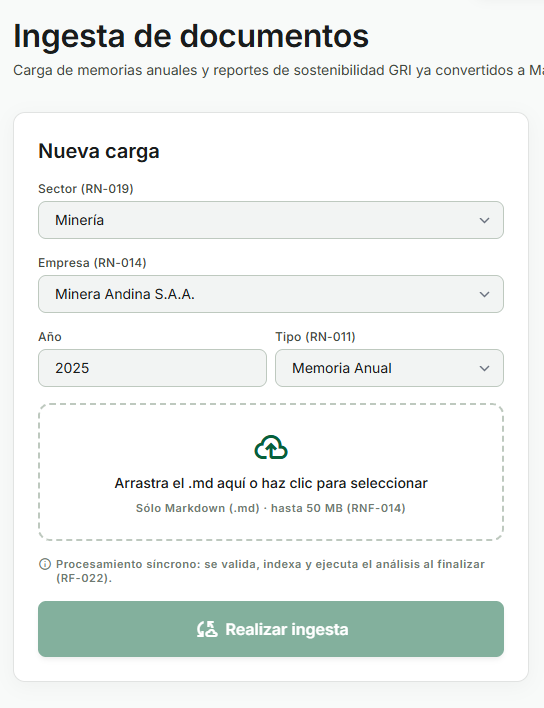
\includegraphics[width=0.62\textwidth]{img/im-026-019.png}}
\figframe{Prototipo --- CU003}{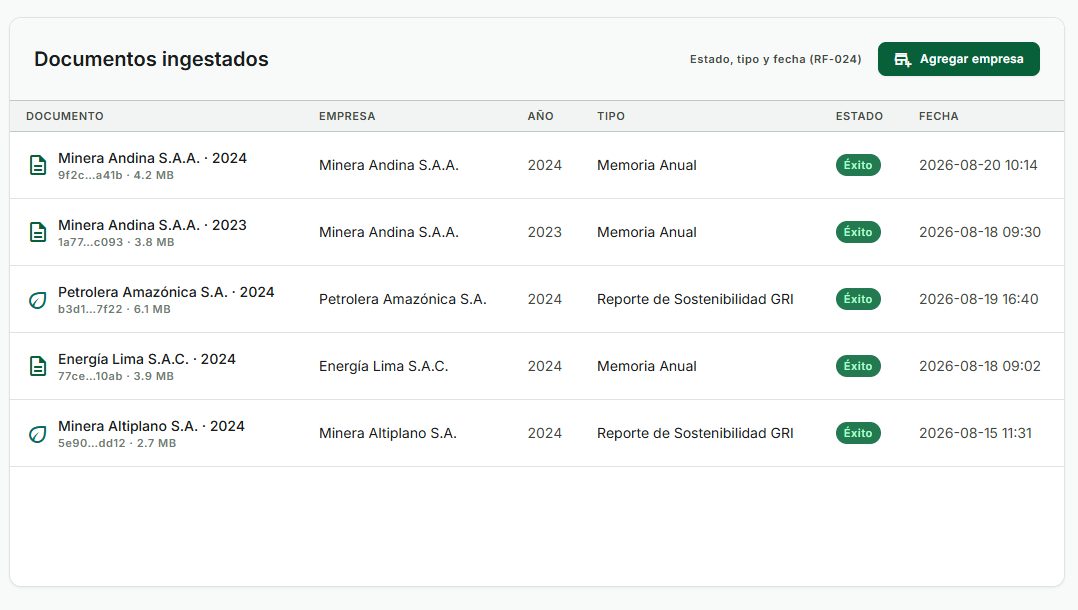
\includegraphics[width=0.92\textwidth]{img/im-026-020.png}}

% ------------------------------- CU004 -------------------------------
\clearpage
\subsubsection*{CU004: Consulta al Asistente de IA (RAG)}
\addcontentsline{toc}{subsubsection}{CU004: Consulta al Asistente de IA (RAG)}
\ficha{
\frow{Descripción}{Este caso de uso permite al Administrador usar al agente de IA para hacerle consultas dependiendo de la empresa y sector específico, también eligiendo el año de los documentos a analizar. Este puede hablar en lenguaje natural con el asistente y responderá de acuerdo a la información de los documentos en el sistema.}
\frow{Actores}{Administrador}
\frow{Precondiciones}{-- El Administrador debe haber iniciado sesión exitosamente.\newline -- Debe encontrarse en el módulo correcto para Consulta de Asistente de IA\newline -- Antes de enviar una consulta, el Administrador debe seleccionar el sector, la empresa y el año. Sin estos datos, el sistema mantiene deshabilitada la opción de consulta.}
\frow{Flujo Básico}{\textbf{Consultas al Asistente de IA}\newline 1. El Administrador accede al módulo de Consulta de Asistente de IA.\newline 2. El Administrador debe elegir el sector, empresa y año para delimitar la información que va a usar el agente de IA. El sistema muestra un mensaje inicial sobre las empresas actualmente en el sistema, y da sugerencias de prompts en lenguaje natural.\newline 3. El Administrador debe ingresar su consulta en lenguaje natural pidiendo la información pertinente de la empresa.\newline 4. El agente de IA debe procesarla, buscando información dentro de los documentos en el sistema.\newline 5. El agente de IA devuelve la respuesta conteniendo la información pedida de la consulta junto con citas para evitar información inventada.}
\frow{Flujo Alternativo}{\textbf{Información no encontrada}\newline Al devolver la información o respuesta pedida, si el documento o información pedida no existe, la IA deberá informar en su respuesta que no existe o no se encuentra, no inventarse información para cumplir con lo pedido.\par\vspace{4pt}\textbf{Consulta fuera del dominio}\newline Si la pregunta no se relaciona con sostenibilidad empresarial, indicadores GRI, sanciones o el contenido de los documentos indexados, el asistente rechaza la consulta e informa que se encuentra fuera del alcance permitido.\par\vspace{4pt}\textbf{Proveedor de IA no disponible}\newline Si el proveedor externo no responde dentro del tiempo máximo establecido, el sistema informa temporalmente la indisponibilidad del asistente. Esta situación no impide utilizar los módulos que no dependen del proveedor de IA (autenticación y gestión de usuarios, catálogo de empresas, reportes de prospección y auditoría).}
\frow{Post Condiciones}{-- Éxito: En la respuesta del agente de IA debe responder a la consulta y devolver la información solicitada.\newline -- Fallo: En su respuesta del agente de IA debe informarle al Administrador que no se encuentra la información solicitada.}
\frow{Restricciones}{-- Solo el rol Administrador tiene la capacidad de interactuar con el agente de IA.}
\frow{Casos de Uso Padre}{---}
}
\figframe{Diagrama de caso de uso --- CU004}{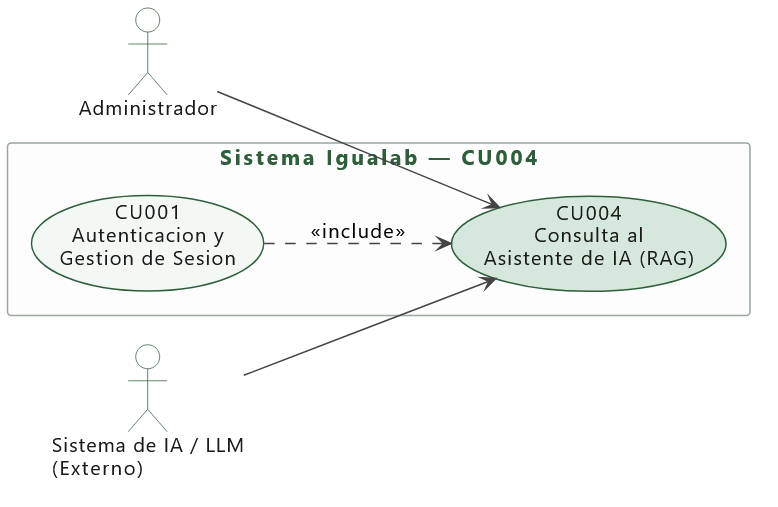
\includegraphics[width=0.72\textwidth]{img/im-028-021.png}}
\figframe{Prototipo --- CU004}{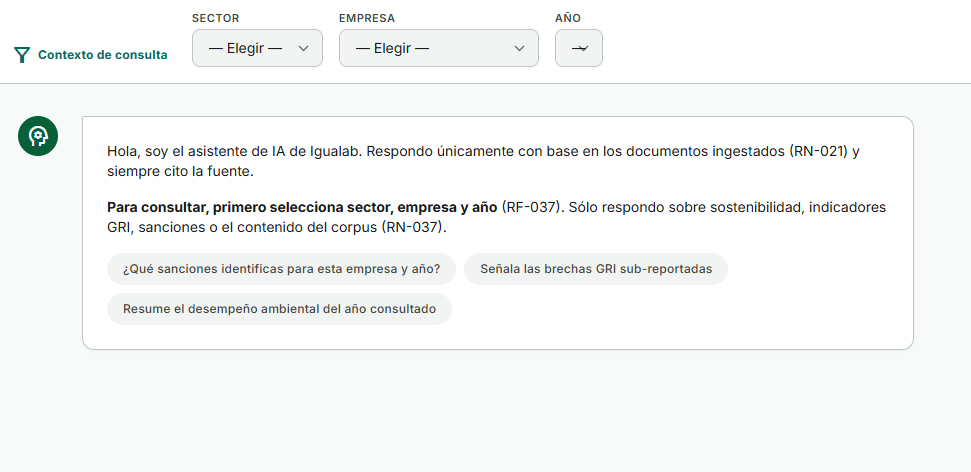
\includegraphics[width=0.85\textwidth]{img/im-028-022.png}}

% ------------------------------- CU005 -------------------------------
\clearpage
\subsubsection*{CU005: Detección de Brechas GRI y Sanciones}
\addcontentsline{toc}{subsubsection}{CU005: Detección de Brechas GRI y Sanciones}
\ficha{
\frow{Descripción}{El Administrador revisa, sobre una empresa con documentos indexados, los códigos GRI y las sanciones detectados por el sistema, y asigna \textbf{manualmente} el estado de cada código (OK, Baja sustancia o Sub-reportado). El sistema no compara el contenido contra el estándar GRI ni infiere el estado: solo detecta los códigos del catálogo presentes y extrae la cita textual de respaldo; las sanciones se toman de menciones explícitas en los documentos.}
\frow{Actores}{Administrador}
\frow{Precondiciones}{-- El Administrador ha iniciado sesión exitosamente y su sesión está vigente.\newline -- La empresa a analizar existe y tiene al menos un documento indexado.\newline -- El análisis GRI se pobló automáticamente al finalizar la ingesta.}
\frow{Flujo Básico}{\textbf{Revisión y validación de brechas}\newline 1. El Administrador accede al módulo de análisis y selecciona la empresa y el año.\newline 2. El sistema muestra los códigos GRI detectados con su \textbf{cita textual} (documento y sección) y las sanciones identificadas.\newline 3. El Administrador revisa cada cita y \textbf{asigna manualmente el estado} del código: OK, Baja sustancia o Sub-reportado.\newline 4. El sistema guarda el cambio con autor, fecha y estado anterior $\rightarrow$ nuevo (historial).\newline 5. El sistema calcula el puntaje ESG a partir de los estados asignados.\newline 6. Cuando todas las filas tienen estado, el sistema habilita la generación del reporte de prospección.}
\frow{Flujo Alternativo}{\textbf{Documentación insuficiente}\newline Si la empresa no tiene documentos indexados, el sistema informa la insuficiencia de datos y no genera resultado.\par\vspace{4pt}\textbf{Sin códigos detectados}\newline Si no se detectó ningún código GRI, el puntaje ESG se muestra como ``no disponible'' (nunca como cero) y se declara la ausencia de hallazgos.\par\vspace{4pt}\textbf{Fallo del proveedor de IA}\newline Si el servicio externo no está disponible, el sistema informa el error sin bloquear el resto de los módulos y permite reintentar.}
\frow{Post Condiciones}{-- Éxito: los estados quedan validados en la tabla del análisis, con su historial, y el resultado queda listo para generar el reporte de prospección.\newline -- Fallo: no se altera la información previamente almacenada y se notifica el motivo.}
\frow{Restricciones}{-- Solo el rol Administrador puede revisar y validar las brechas y sanciones.\newline -- El sistema no infiere ni calcula el estado; la asignación es 100\,\% manual (RN-029, RN-030).\newline -- Toda brecha y sanción reportada debe citar su fuente (documento y sección).\newline -- No se consultan fuentes externas al corpus del sistema.}
\frow{Casos de Uso Padre}{CU003 --- Ingesta de Documentos (memorias y reportes GRI)}
}
\figframe{Diagrama de caso de uso --- CU005}{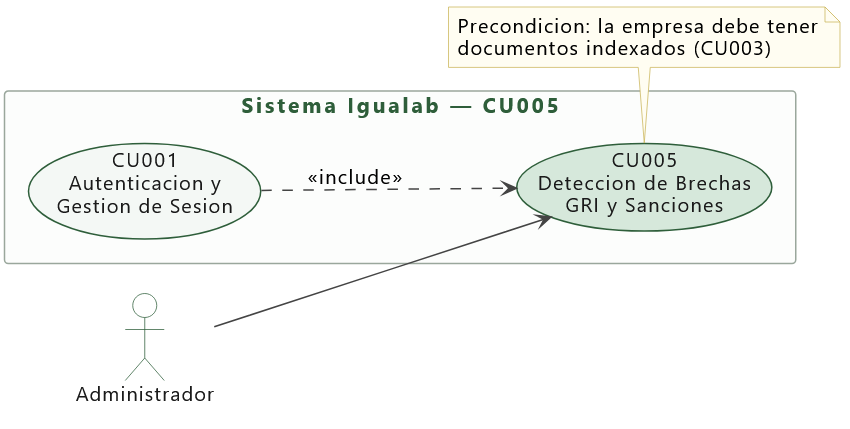
\includegraphics[width=0.72\textwidth]{img/im-030-024.png}}
\figframe{Prototipo --- CU005}{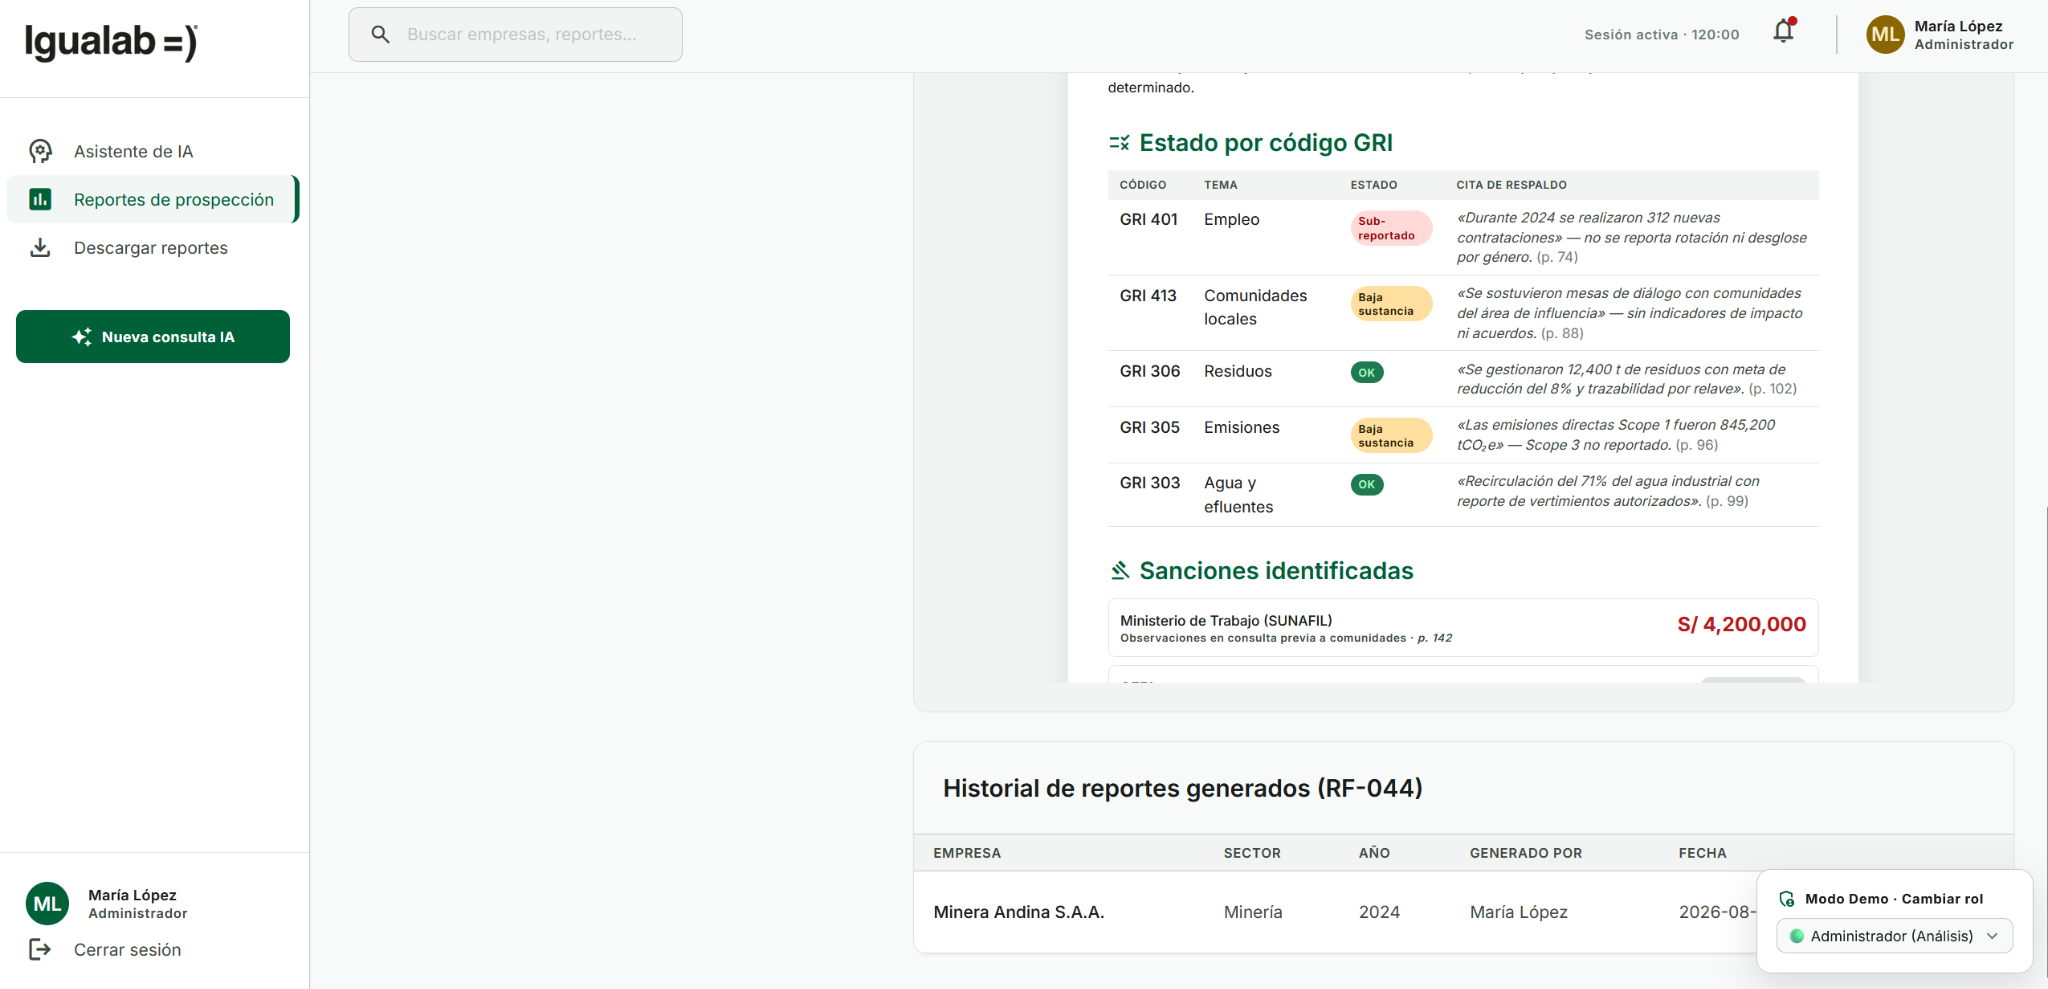
\includegraphics[width=0.9\textwidth]{img/im-031-025.png}}

% ------------------------------- CU006 -------------------------------
\clearpage
\subsubsection*{CU006: Generación de Reportes de Prospección (PDF)}
\addcontentsline{toc}{subsubsection}{CU006: Generación de Reportes de Prospección (PDF)}
\ficha{
\frow{Descripción}{Este caso de uso permite al Administrador generar un reporte de prospección para una empresa y un año determinados. El reporte se construye a partir de los resultados GRI revisados y validados, las citas de respaldo, las sanciones identificadas y el puntaje ESG. La generación no invoca al proveedor de inteligencia artificial.}
\frow{Actores}{Administrador}
\frow{Precondiciones}{-- El Administrador debe mantener una sesión vigente.\newline -- La empresa y el año seleccionados deben contar con al menos un documento indexado.\newline -- Los resultados GRI requeridos para el reporte deben haber sido revisados y validados manualmente.\newline -- No debe existir otro reporte generado para la misma empresa y año.}
\frow{Flujo Básico}{\textbf{Generar reportes de prospección}\newline 1. El Administrador accede al módulo de reportes de prospección.\newline 2. Es necesario llenar los datos del sector, empresa y año del cual se generará dicho documento.\newline 3. Tiene la capacidad de hacer una vista previa del documento previa a la generación y descarga del documento.\newline 4. Puede generar y descargar el documento de reporte de prospección.}
\frow{Flujo Alternativo}{\textbf{Generar reporte de un año que no haya documento}\newline El sistema no habilita la vista previa, generación o descarga del documento ya que no hay posibilidad de hacerlo.\par\vspace{4pt}\textbf{Reporte existente}\newline Si ya existe un reporte para la misma empresa y año, el sistema no genera uno nuevo y permite visualizar o descargar el reporte existente.}
\frow{Post Condiciones}{-- Éxito: El documento es generado, capaz de visualizarse y descargarse.\newline -- Fallo: El documento no es capaz de ser generado si el documento no existe.}
\frow{Restricciones}{-- Solo el rol Administrador puede acceder a este módulo.\newline -- El documento del cual se hará el reporte debe existir en el sistema.\newline -- Solo puede existir un reporte de prospección por combinación de empresa y año.}
\frow{Casos de Uso Padre}{CU005 --- Detección de Brechas GRI y Sanciones}
}
\figframe{Diagrama de caso de uso --- CU006}{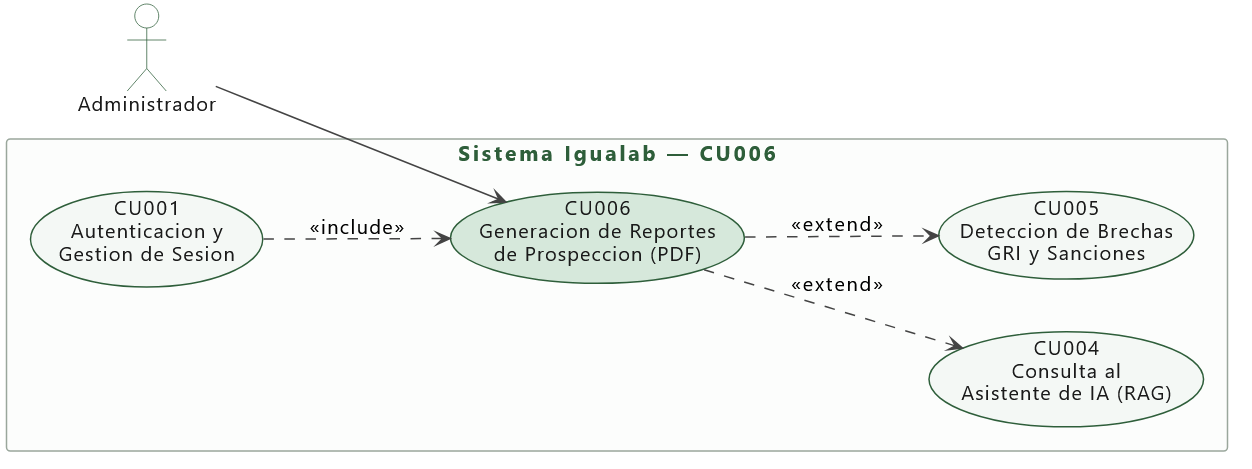
\includegraphics[width=0.85\textwidth]{img/im-032-027.png}}
\figframe{Prototipo --- CU006}{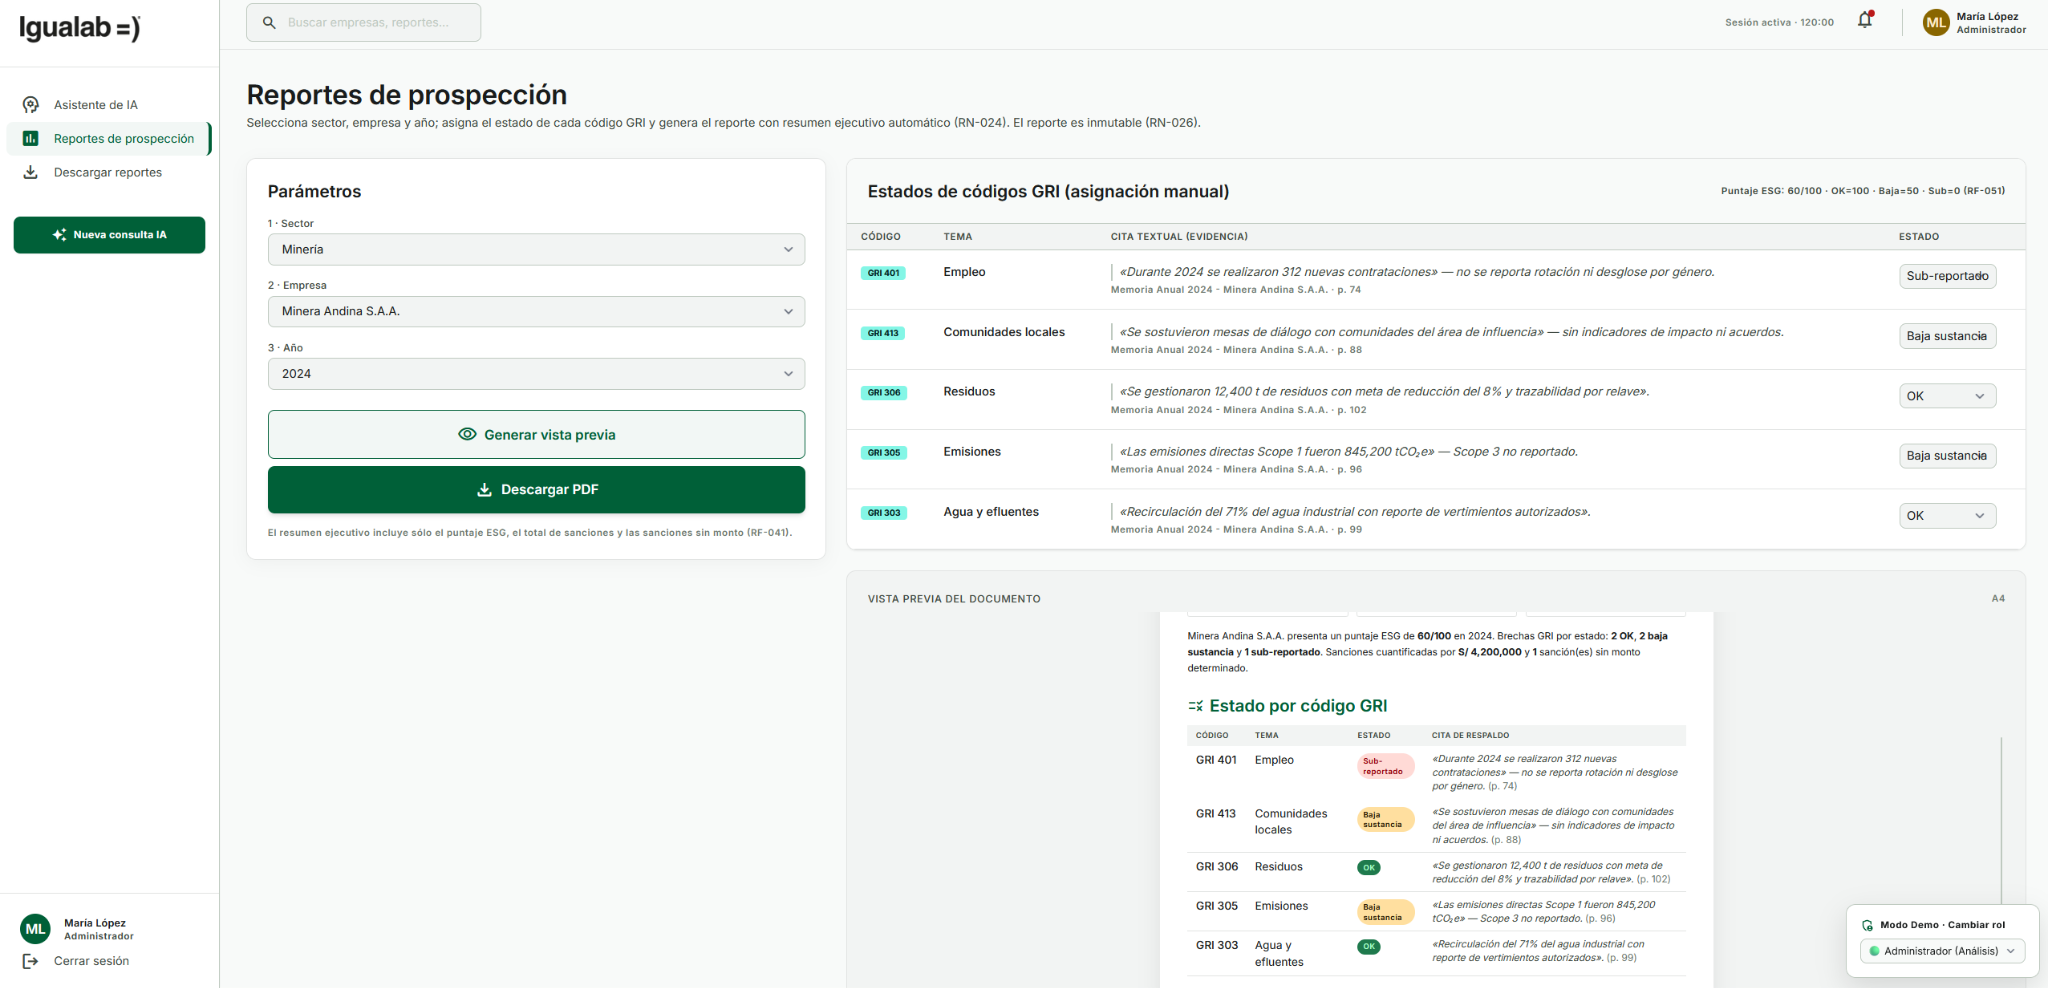
\includegraphics[width=0.9\textwidth]{img/im-032-028.png}}

% ------------------------------- CU007 -------------------------------
\clearpage
\subsubsection*{CU007: Auditoría de Eventos del Sistema}
\addcontentsline{toc}{subsubsection}{CU007: Auditoría de Eventos del Sistema}
\ficha{
\frow{Descripción}{El sistema registra automáticamente los eventos sensibles (inicios de sesión, cambios o transferencias de rol, ingesta de documentos y generación de reportes) con el usuario, la acción y la fecha, y permite al SuperAdmin consultarlos y filtrarlos para garantizar la trazabilidad y el cumplimiento de las políticas de seguridad.}
\frow{Actores}{SuperAdmin}
\frow{Precondiciones}{-- El SuperAdmin ha iniciado sesión exitosamente y su sesión está vigente\newline -- Para la consulta, existe al menos un evento registrado.}
\frow{Flujo Básico}{1. Cada vez que ocurre un evento sensible (login, cambio/transferencia de rol, ingesta, generación de reporte), el sistema lo registra automáticamente con usuario, acción, entidad afectada y fecha/hora.\newline 2. El SuperAdmin accede al módulo de auditoría.\newline 3. El sistema muestra el registro de eventos.\newline 4. El SuperAdmin aplica filtros (por usuario, tipo de evento o rango de fechas) y consulta los eventos de interés.}
\frow{Flujo Alternativo}{\textbf{Sin coincidencias}\newline En el paso 4, ningún evento cumple el filtro aplicado. El sistema informa que no hay eventos para ese criterio.\par\vspace{4pt}\textbf{Acceso no autorizado}\newline Si un rol distinto de SuperAdmin intenta acceder al módulo, el sistema deniega el acceso (HTTP 403) y registra el intento.}
\frow{Post Condiciones}{-- Los eventos sensibles quedan registrados de forma persistente y son consultables por el SuperAdmin.\newline -- La consulta no modifica los registros; el log es de solo lectura al consultarse.}
\frow{Restricciones}{-- Solo el rol SuperAdmin tiene acceso a esta sección.\newline -- La información registrada es inmutable.}
\frow{Casos de Uso Padre}{---}
}
\figframe{Diagrama de caso de uso --- CU007}{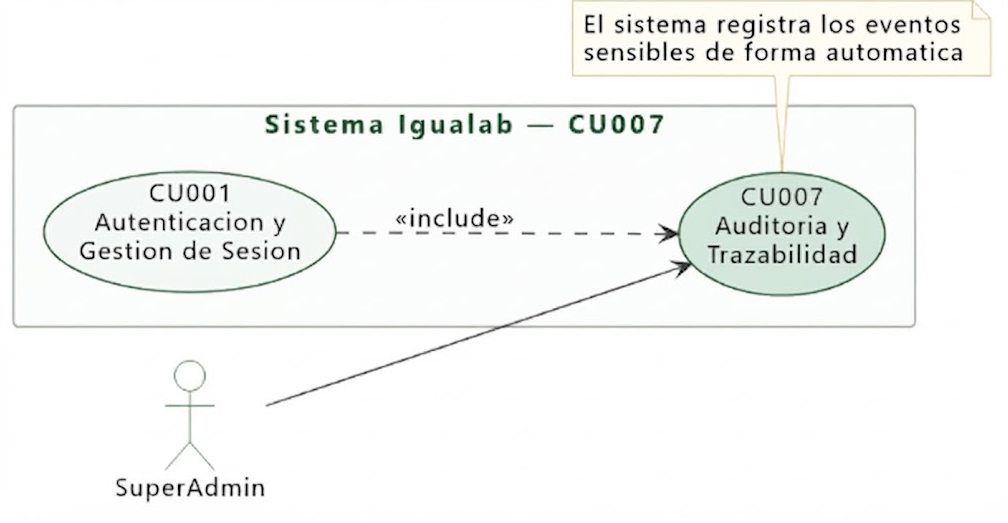
\includegraphics[width=0.72\textwidth]{img/im-033-030.png}}
\figframe{Prototipo --- CU007}{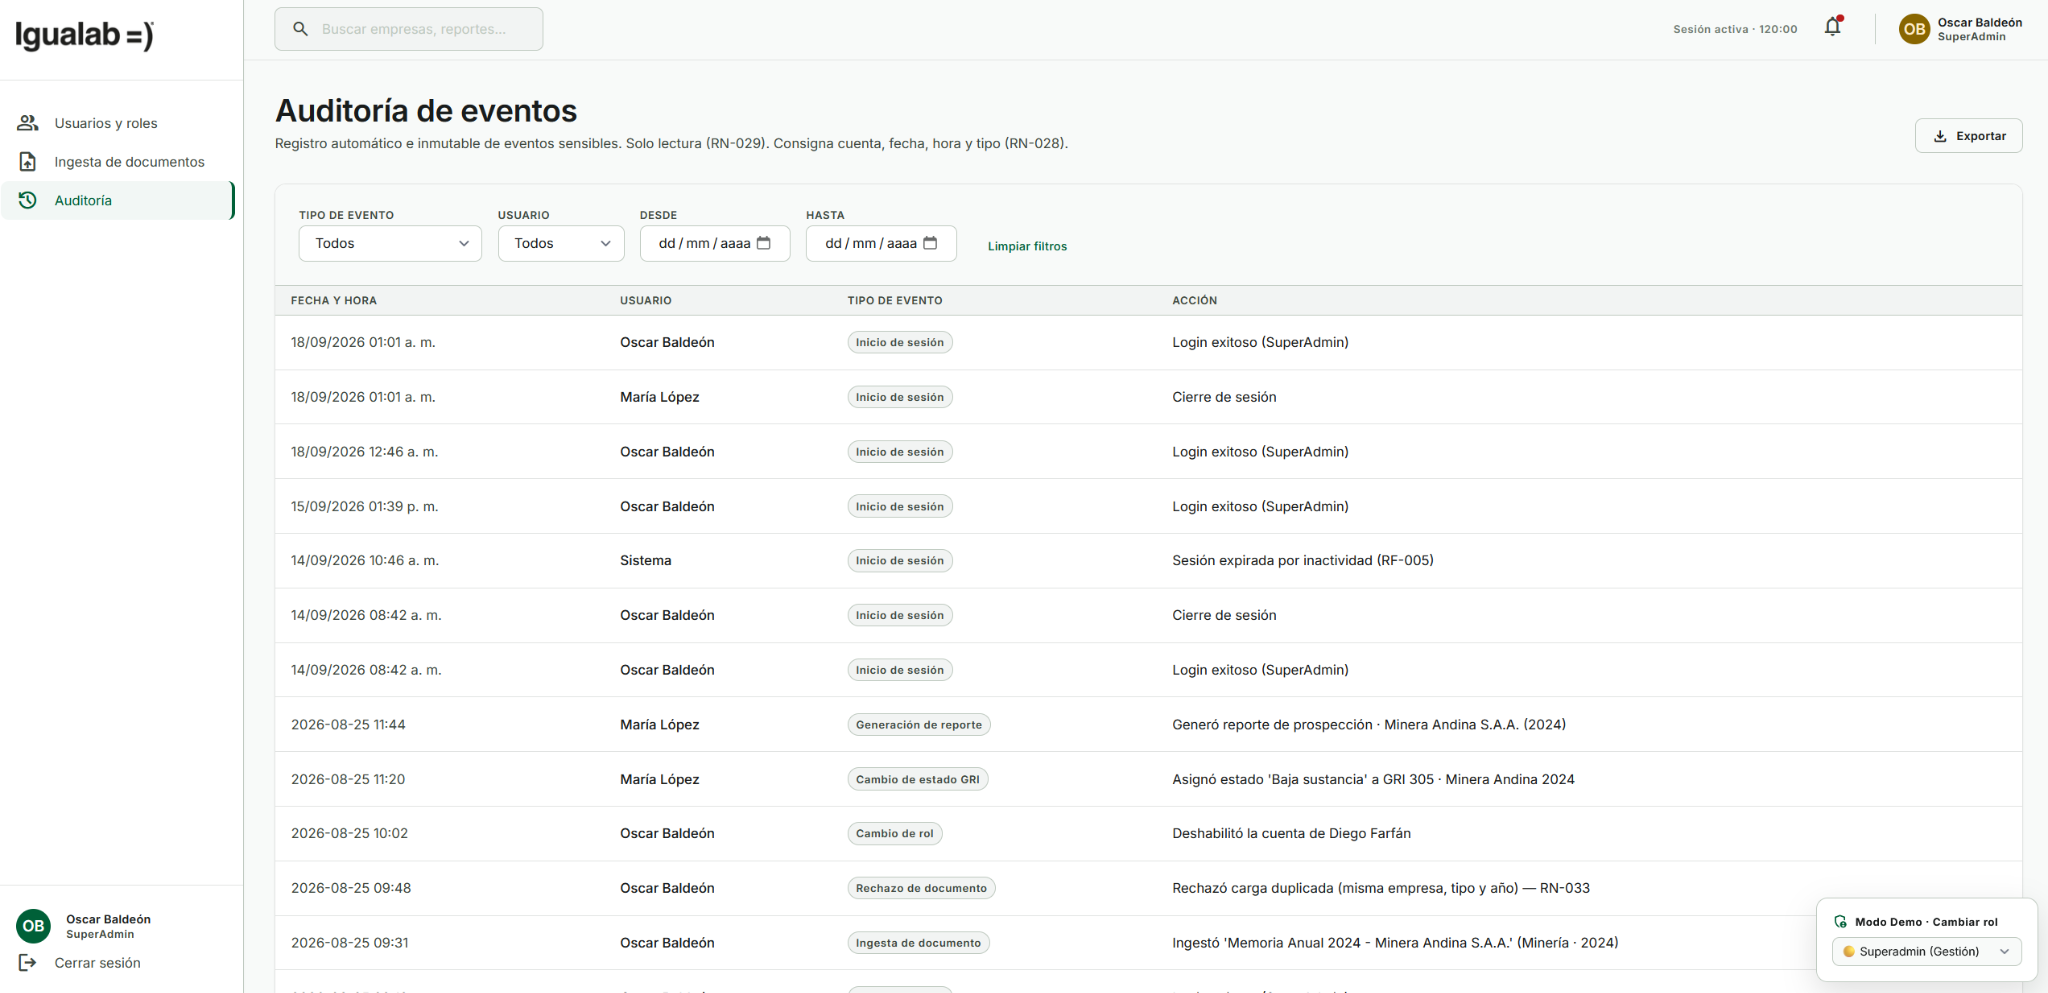
\includegraphics[width=0.9\textwidth]{img/im-034-031.png}}

% ---------------------------- 7.3 SECUENCIA --------------------------
\clearpage
\subsection{Diagrama de Secuencia}
\addcontentsline{toc}{subsubsection}{Autenticación y Gestión de Sesión}
\noindent\textbf{Caso de uso:} Autenticación y Gestión de Sesión
\begin{center}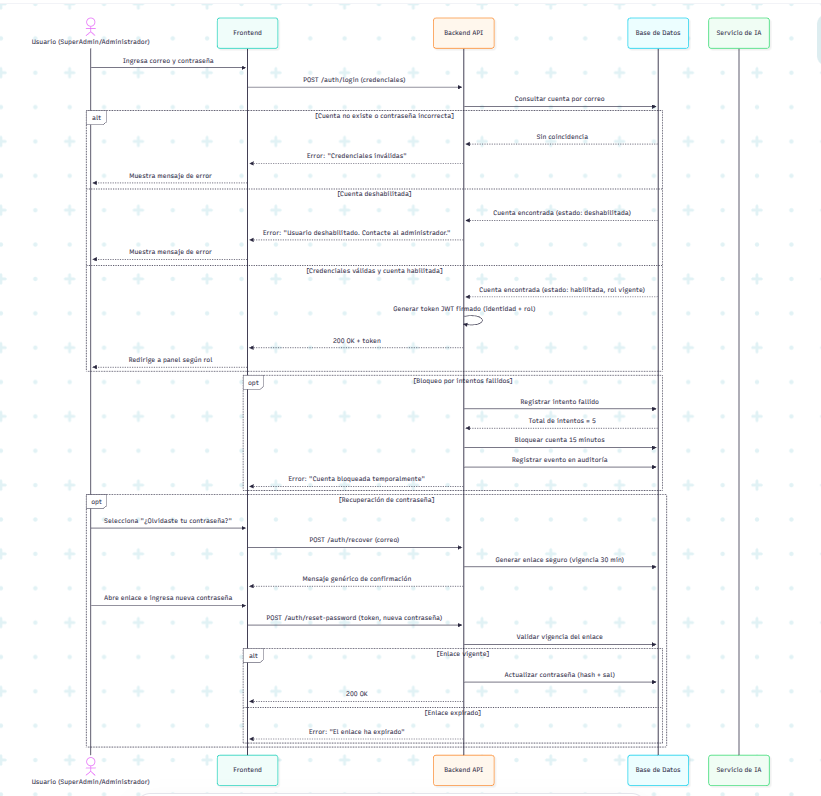
\includegraphics[width=0.85\textwidth]{img/im-034-033.png}\end{center}

\addcontentsline{toc}{subsubsection}{Gestión de Usuarios}
\noindent\textbf{Caso de uso:} Gestión de Usuarios
\begin{center}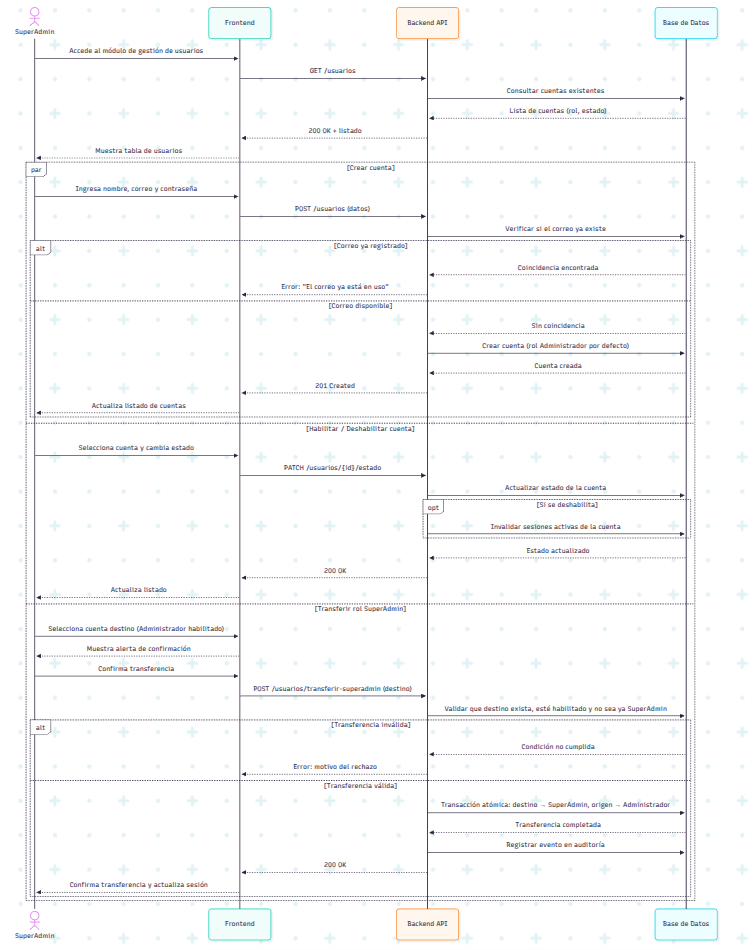
\includegraphics[width=0.85\textwidth]{img/im-035-034.png}\end{center}

\addcontentsline{toc}{subsubsection}{Ingesta de documentos (análisis GRI)}
\noindent\textbf{Caso de uso:} Ingesta de documentos (análisis GRI)
\begin{center}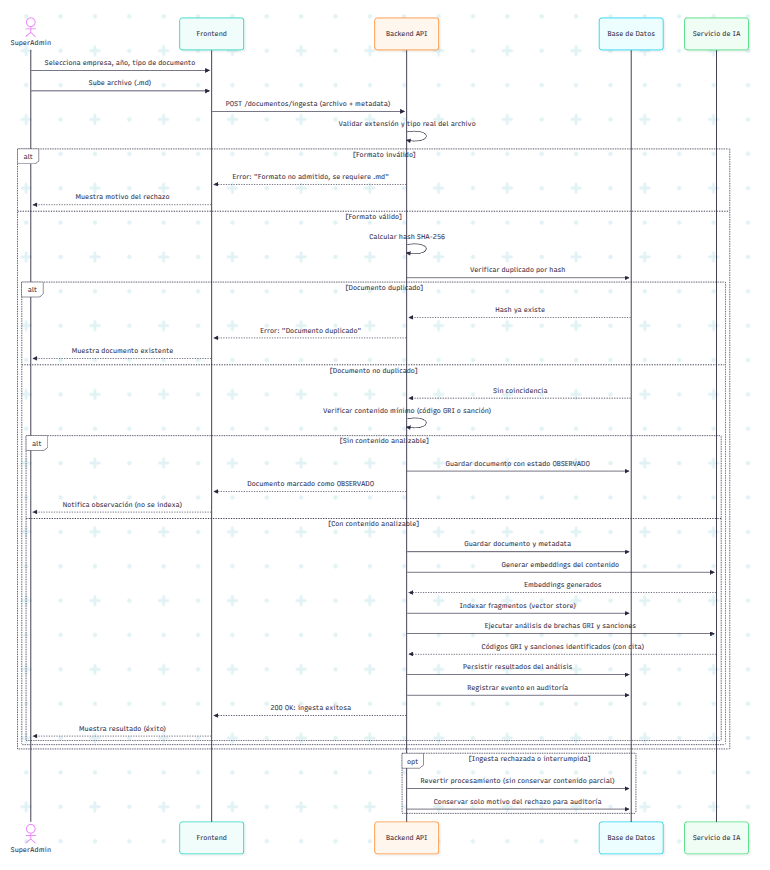
\includegraphics[width=0.85\textwidth]{img/im-036-035.png}\end{center}

\addcontentsline{toc}{subsubsection}{Consulta al Asistente de IA}
\noindent\textbf{Caso de uso:} Consulta al Asistente de IA
\begin{center}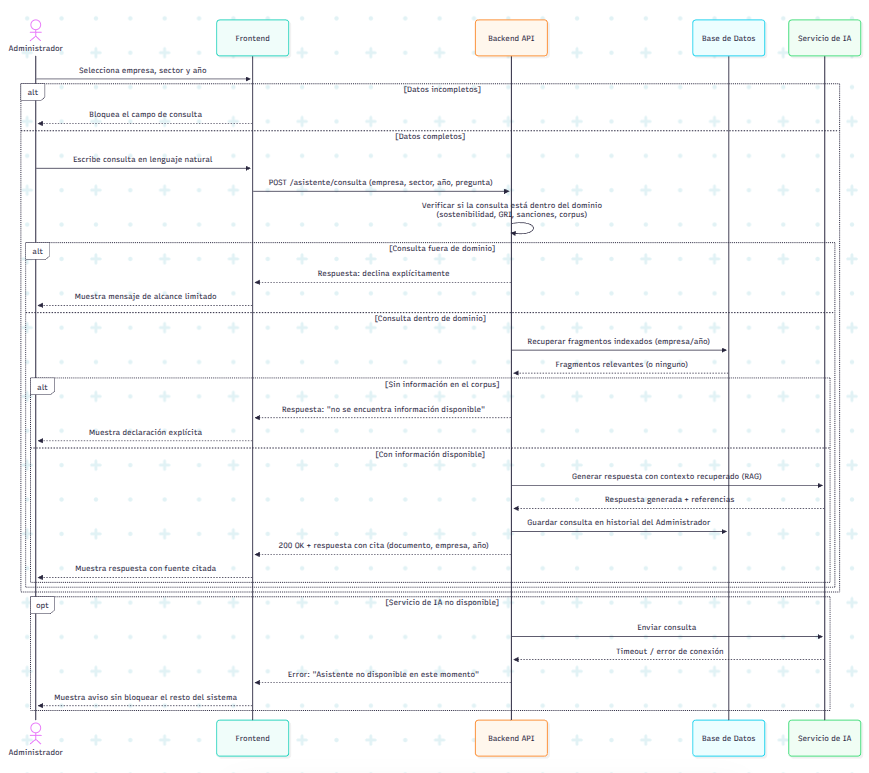
\includegraphics[width=0.85\textwidth]{img/im-037-036.png}\end{center}

\addcontentsline{toc}{subsubsection}{Detección de Brechas GRI y Sanciones}
\noindent\textbf{Caso de uso:} Detección de Brechas GRI y Sanciones
\begin{center}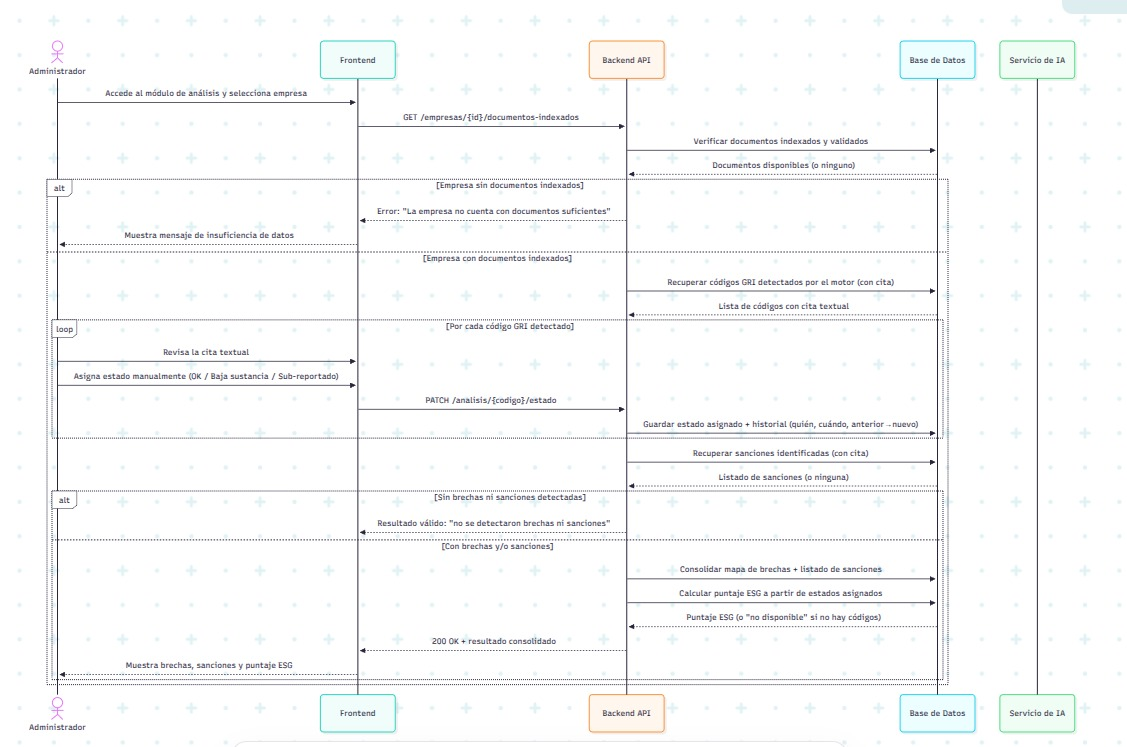
\includegraphics[width=0.85\textwidth]{img/diagrama-secuencia-CU005.jpeg}\end{center}

\addcontentsline{toc}{subsubsection}{Generación de Reportes de Prospección}
\noindent\textbf{Caso de uso:} Generación de Reportes de Prospección
\begin{center}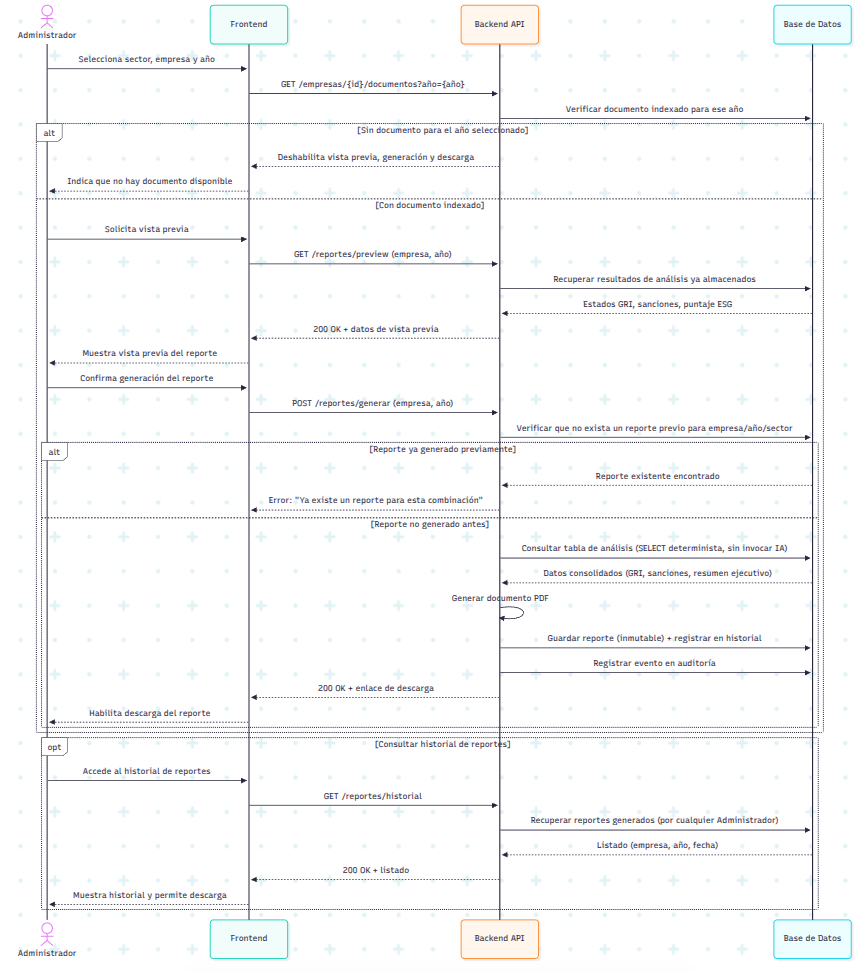
\includegraphics[width=0.85\textwidth]{img/im-038-037.png}\end{center}

\addcontentsline{toc}{subsubsection}{Auditoría de Eventos del Sistema}
\noindent\textbf{Caso de uso:} Auditoría de Eventos del Sistema
\begin{center}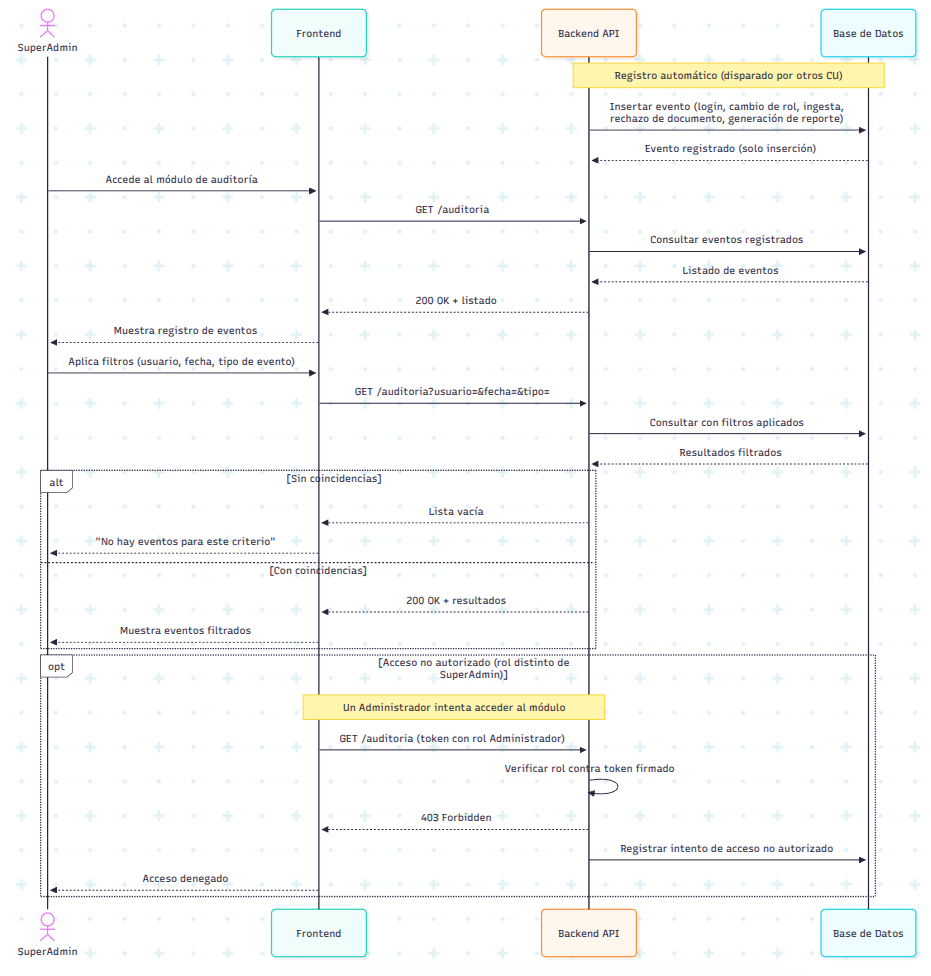
\includegraphics[width=0.85\textwidth]{img/im-039-038.png}\end{center}

% ------------------------------- 7.4 RF -------------------------------
\clearpage
\subsection{Requerimientos Funcionales}
Los requerimientos funcionales se redactan de forma atómica, verificable, comprensible y libre de implementación, y cada uno se deriva de una o varias reglas de negocio (RN). Se detallan a continuación.

La numeración de los requerimientos funcionales presentada en esta versión constituye la línea base vigente del proyecto. Cualquier artefacto anterior, caso de prueba o elemento del backlog deberá actualizar sus referencias para mantener la trazabilidad con esta versión.

\begingroup\small
% ====================================================================
%  7.4 · REQUERIMIENTOS FUNCIONALES (atómicos, derivados de RN)
% ====================================================================
\begin{longtable}{|C{1.1cm}|L{6.6cm}|L{3.1cm}|C{1.6cm}|C{1.8cm}|}
\hline
\thd{N\textdegree} & \thd{Descripción del Requerimiento Funcional} & \thd{Reglas de Negocio} & \thd{Prioridad} & \thd{Analista} \\
\hline
\endfirsthead
\hline
\thd{N\textdegree} & \thd{Descripción del Requerimiento Funcional} & \thd{Reglas de Negocio} & \thd{Prioridad} & \thd{Analista} \\
\hline
\endhead
RF-001 & Autenticar a los usuarios con correo y contraseña. & RN-004, RN-007, RN-011 & MUST HAVE & C. Ordinola \\
\hline
RF-002 & Permitir la recuperación de contraseña mediante un enlace seguro de un solo uso. & RN-010, RN-011 & MUST HAVE & C. Ordinola \\
\hline
RF-003 & Permitir al usuario cambiar su propia contraseña estando autenticado. & RN-011 & NICE TO HAVE & L. Millones \\
\hline
RF-004 & Gestionar la sesión del usuario (expiración por inactividad, cierre de sesión y rol vigente). & RN-005, RN-013 & MUST HAVE & L. Millones \\
\hline
RF-005 & Bloquear temporalmente la cuenta tras 5 intentos fallidos consecutivos. & RN-012 & MUST HAVE & C. Ordinola \\
\hline
RF-006 & Crear cuentas de Administrador con nombre, correo y contraseña. & RN-002, RN-007, RN-008 & MUST HAVE & C. Ordinola \\
\hline
RF-007 & Habilitar y deshabilitar cuentas de Administrador. & RN-002, RN-005 & MUST HAVE & L. Millones \\
\hline
RF-008 & Transferir el rol SuperAdmin a una cuenta de Administrador habilitada. & RN-002, RN-006, RN-009 & MUST HAVE & L. Millones \\
\hline
RF-009 & Listar las cuentas existentes con su rol y estado. & RN-001, RN-003 & NICE TO HAVE & C. Ordinola \\
\hline
RF-010 & Registrar empresas asociándolas a un sector. & RN-014, RN-015, RN-016 & MUST HAVE & C. Ordinola \\
\hline
RF-011 & Activar y desactivar empresas del catálogo. & RN-017 & NICE TO HAVE & L. Millones \\
\hline
RF-012 & Cargar documentos Markdown (.md) asociándolos a una empresa, un año y un tipo. & RN-018, RN-019, RN-020, RN-022 & MUST HAVE & C. Ordinola \\
\hline
RF-013 & Validar el documento cargado (formato, tamaño hasta 50 MB y contenido mínimo). & RN-021, RN-025 & MUST HAVE & C. Ordinola \\
\hline
RF-014 & Rechazar documentos duplicados por contenido o por empresa, año y tipo. & RN-023, RN-024 & MUST HAVE & L. Millones \\
\hline
RF-015 & Procesar la ingesta de forma síncrona mostrando el progreso. & RN-026 & MUST HAVE & L. Millones \\
\hline
RF-016 & Indexar el documento para el asistente (fragmentos y embeddings). & RN-018, RN-025 & MUST HAVE & C. Ordinola \\
\hline
RF-017 & Ejecutar el análisis GRI y de sanciones al finalizar la ingesta. & RN-026, RN-027, RN-028 & MUST HAVE & C. Ordinola \\
\hline
RF-018 & Detectar los códigos GRI presentes y extraer su cita textual. & RN-027, RN-028 & MUST HAVE & L. Millones \\
\hline
RF-019 & Permitir al Administrador asignar manualmente el estado de cada código GRI. & RN-029, RN-030 & MUST HAVE & L. Millones \\
\hline
RF-020 & Identificar las sanciones mencionadas en los documentos. & RN-031 & MUST HAVE & C. Ordinola \\
\hline
RF-021 & Calcular el puntaje ESG de una empresa y un año. & RN-032 & MUST HAVE & C. Ordinola \\
\hline
RF-022 & Consultar el listado de documentos ingestados con su estado. & RN-022, RN-025 & NICE TO HAVE & L. Millones \\
\hline
RF-023 & Consultar al asistente en lenguaje natural sobre el corpus indexado. & RN-033, RN-034, RN-037 & MUST HAVE & C. Ordinola \\
\hline
RF-024 & Recibir respuestas con citas y con el dominio restringido a sostenibilidad. & RN-034, RN-035, RN-036 & MUST HAVE & L. Millones \\
\hline
RF-025 & Generar el reporte de prospección en PDF a partir de los resultados validados. & RN-038, RN-039, RN-040 & MUST HAVE & C. Ordinola \\
\hline
RF-026 & Visualizar y descargar el historial de reportes de prospección. & RN-041 & NICE TO HAVE & L. Millones \\
\hline
RF-027 & Visualizar las brechas GRI de una empresa con su cita de respaldo. & RN-028, RN-034 & MUST HAVE & C. Ordinola \\
\hline
RF-028 & Consultar y filtrar los eventos de auditoría. & RN-042, RN-043, RN-044, RN-045 & NICE TO HAVE & L. Millones \\
\hline
\end{longtable}

\endgroup

% ------------------------------- 7.5 RNF ------------------------------
\subsection{Requerimientos No Funcionales}
Los requerimientos no funcionales definen las restricciones de calidad bajo las cuales opera el sistema y se derivan de las reglas de negocio (RN) y de los requerimientos funcionales (RF) a los que califican. Se presentan categorizados.

\begingroup\small
% ====================================================================
%  7.5 · REQUERIMIENTOS NO FUNCIONALES (categorizados · Deriva de RN/RF)
% ====================================================================
\begin{longtable}{|C{1.7cm}|L{2.9cm}|L{6.4cm}|L{3.4cm}|}
\hline
\thd{N\textdegree} & \thd{Categoría} & \thd{Descripción del Requerimiento No Funcional} & \thd{Deriva de} \\
\hline
\endfirsthead
\hline
\thd{N\textdegree} & \thd{Categoría} & \thd{Descripción del Requerimiento No Funcional} & \thd{Deriva de} \\
\hline
\endhead
RNF-001 & Seguridad & Las contraseñas deben tener un mínimo de 8 caracteres, con al menos una mayúscula, una minúscula, un dígito y un carácter especial, y no pueden coincidir con el correo de la cuenta. & RF-001, RN-011 \\
\hline
RNF-002 & Seguridad & Las contraseñas se almacenan mediante una función de hash de un solo sentido con sal única por usuario, nunca en texto plano. & RF-001, RN-011 \\
\hline
RNF-003 & Seguridad & La identidad de la cuenta se obtiene exclusivamente del token firmado (JWT), nunca de parámetros de la petición. & RF-001, RF-004, RN-003 \\
\hline
RNF-004 & Seguridad & La clave utilizada para firmar los tokens JWT se almacena fuera del código fuente mediante variables de entorno o secretos del ambiente. Su rotación no requiere modificar el código y se aplica mediante una actualización segura de la configuración y un reinicio controlado del servicio. & RF-001 \\
\hline
RNF-005 & Seguridad & La autorización se evalúa en cada endpoint, con independencia de lo que exponga la interfaz. & RN-003 \\
\hline
RNF-006 & Seguridad & La revocación de la sesión y la vigencia del rol se verifican en cada petición. & RF-004, RN-005, RN-013 \\
\hline
RNF-007 & Seguridad & El tipo real del archivo se valida en el servidor, sin confiar en la extensión declarada. & RF-013, RN-018 \\
\hline
RNF-008 & Seguridad & Las respuestas de recuperación y el mensaje de error de autenticación son idénticos para toda cuenta (no revelan su existencia). & RF-001, RF-002, RN-010 \\
\hline
RNF-009 & Seguridad & El token del enlace de recuperación se genera con un generador de números aleatorios criptográficamente seguro. & RF-002, RN-010 \\
\hline
RNF-010 & Seguridad & El contenido recuperado del corpus se trata como datos dentro del prompt, nunca como instrucciones (protección ante \emph{prompt injection}). & RF-024, RN-033, RN-034 \\
\hline
RNF-011 & Integridad & La unicidad documental por contenido emplea el algoritmo de hash SHA-256. & RF-014, RN-024 \\
\hline
RNF-012 & Integridad & La transferencia del rol SuperAdmin se ejecuta en una transacción única; un fallo parcial revierte toda la operación. & RF-008, RN-009 \\
\hline
RNF-013 & Integridad & La unicidad del SuperAdmin se garantiza mediante una restricción de integridad en la base de datos, además de la validación en la aplicación. & RN-002 \\
\hline
RNF-014 & Integridad & El modelo de datos distingue entre un valor no determinado y un valor igual a cero. & RN-031, RN-032 \\
\hline
RNF-015 & Integridad & El contenido de los documentos se procesa y almacena en UTF-8, preservando tildes y la letra «ñ» sin alteración. & RF-012, RF-016 \\
\hline
RNF-016 & Rendimiento & El sistema debe procesar la ingesta e indexación de un documento de hasta 50 MB dentro del tiempo máximo validado mediante pruebas de rendimiento, considerando la latencia y los límites del proveedor externo de embeddings. & RF-015 \\
\hline
RNF-017 & Rendimiento & El sistema debe registrar por separado el tiempo de procesamiento interno y el tiempo de respuesta del proveedor externo. Bajo condiciones normales, la respuesta completa del asistente no debe superar el límite definido durante las pruebas de rendimiento. & RF-023 \\
\hline
RNF-018 & Rendimiento & Las llamadas al proveedor de IA tienen un tiempo máximo de espera de 1 minuto, tras el cual la operación se reporta como indisponible. & RF-023 \\
\hline
RNF-019 & Disponibilidad & La indisponibilidad del proveedor de IA no degrada los módulos de gestión, ingesta, reportes de prospección ni auditoría. & RF-024, RN-033 \\
\hline
RNF-020 & Capacidad & El sistema admite y procesa documentos de hasta 50 MB por cada operación de ingesta. & RF-013, RN-021 \\
\hline
RNF-021 & Disponibilidad & El sistema ofrece una disponibilidad de al menos el 95\,\% en horario laboral (lun–vie, 8:00–20:00, hora de Perú). & Transversal \\
\hline
RNF-022 & Trazabilidad & Los registros de auditoría se almacenan en estructuras de solo inserción (\emph{append-only}), sin actualización ni eliminación. & RN-044 \\
\hline
RNF-023 & Trazabilidad & El registro de auditoría conserva sus entradas durante todo el periodo de operación del sistema. & RN-044 \\
\hline
RNF-024 & Trazabilidad & La fecha y hora de la auditoría se almacenan en UTC y se convierten a \emph{America/Lima} solo en la presentación. & RN-043 \\
\hline
RNF-025 & Trazabilidad & Todo fragmento indexado conserva la referencia a su documento de origen y a su ubicación dentro de él. & RF-016, RN-034 \\
\hline
RNF-026 & Mantenibilidad & El catálogo de 40 códigos GRI se carga mediante un script de inicialización versionado, garantizando el mismo catálogo en todos los ambientes. & RN-027 \\
\hline
RNF-027 & Mantenibilidad & El sistema integra al proveedor de IA mediante una interfaz estandarizada, de modo que cambiar de modelo o proveedor no obliga a rediseñar. & RF-023 \\
\hline
RNF-028 & Usabilidad & Durante la ingesta síncrona el sistema mantiene informado al usuario del progreso de la operación. & RF-015, RN-026 \\
\hline
RNF-029 & Usabilidad & Los mensajes de estado y de rechazo se presentan en español claro y accionable, indicando el motivo. & RF-013 \\
\hline
RNF-030 & Continuidad & Se realizan copias de seguridad diarias de la base de datos (incluido el índice vectorial) y de los documentos \texttt{.md} originales. & RF-016 \\
\hline
\end{longtable}

\endgroup
